\section{Coral Dev-Board}
\label{sec:hard-devboard}
Nowadays some manufacturers replace the GPU for a TPU, a Tensor Processing Unit.
Driven by the exponential interest for deep learning in different field such as
research, industries, robotics. The Coral Dev Board is a single-board computer
that contains an Edge TPU coprocessor. It's ideal for prototyping new projects
that demand fast on-device inferencing for machine learning models. Coral Dev
Board cannot train a neural network because the TPU is specific designed to work
with special pre-compiled model and to be small and energy efficient.
%
\begin{figure}[htb]
	\centering
	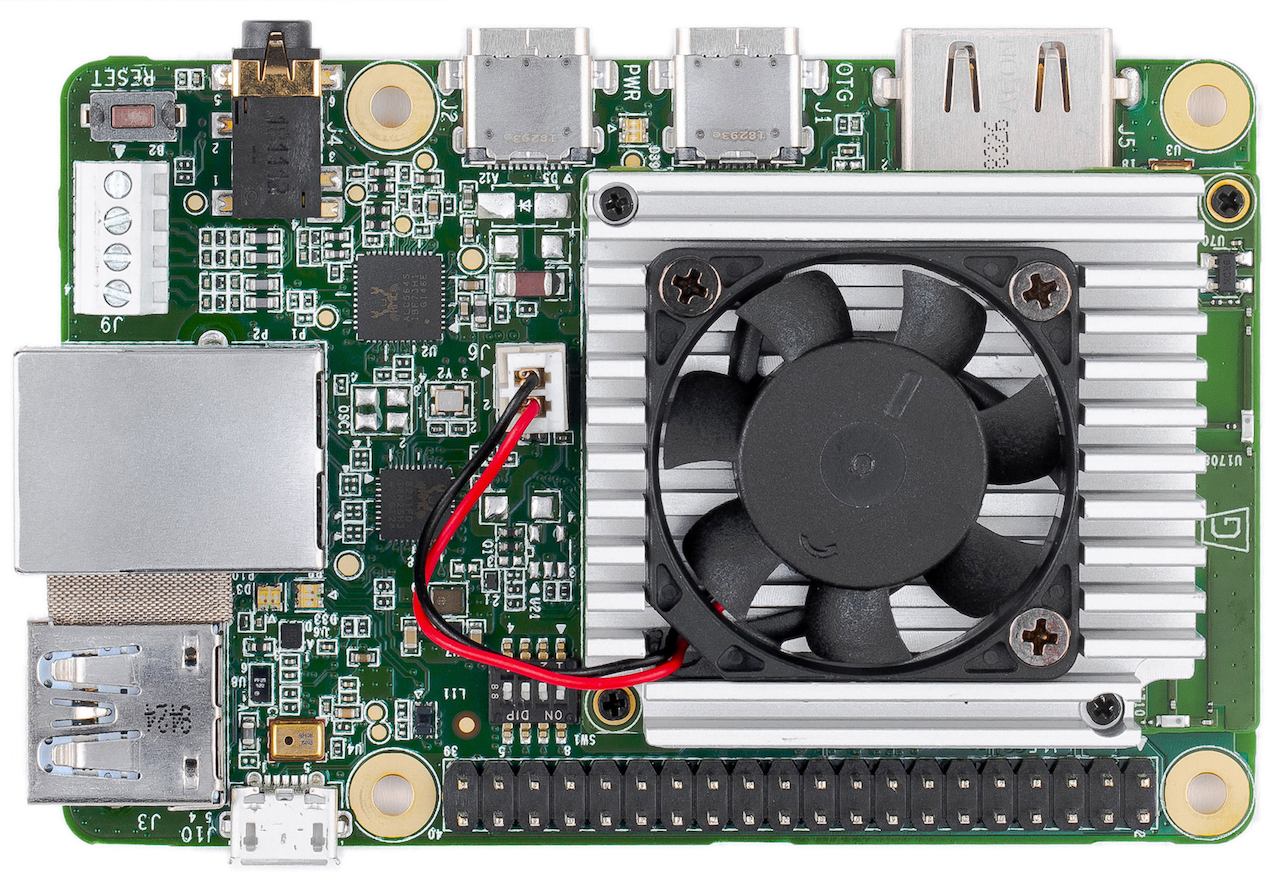
\includegraphics[width=0.75\textwidth]{devboard-dimensions.jpg}
	\captionsource{Coral Dev Board.}{
	\href{https://coral.ai/docs/dev-board/get-started/}{https://coral.ai/docs/dev-board/get-started/}}
	\label{fig:dev-board}
\end{figure}
%
\subsection{Overview}
\label{ssec:hard-devboard-overview}
The Coral Dev Board is a single-board computer that's ideal when you need to
perform fast machine learning (ML) inferencing in a small form factor. You can
use the Dev Board to prototype your embedded system and then scale to production
using the on-board Coral System-on-Module (SoM) combined with your custom PCB
hardware. The SoM provides a fully-integrated system, including NXP's iMX 8M
system-on-chip (SoC), eMMC memory, LPDDR4 RAM, Wi-Fi, and Bluetooth, but its
unique power comes from Google's Edge TPU coprocessor. The Edge TPU is a small
ASIC designed by Google that provides high performance ML inferencing with a low
power cost. For example, it can execute state-of-the-art mobile vision models
such as MobileNet v2 at almost 400 FPS, in a power efficient manner. 
The baseboard provides all the peripheral connections you need to prototype a
project, including USB 2.0/3.0 ports, DSI display interface, CSI-2 camera
interface, Ethernet port, speaker terminals, and a 40-pin I/O header. \hfill \break
Key benefits of the Dev Board:
\begin{itemize}
	\item High-speed and low-power ML inferencing (4 TOPS @ 2 \si{\watt})
	\item A complete Linux system (running Mendel, a Debian derivative)
	\item Prototyping and evaluation board for the small Coral SoM (40 x 48 \si{\milli\meter})
\end{itemize}
%
\begin{table}[htb]
	\centering
	\begin{tabular}{l}
		\hline
		\rowcolor{aliceblue!85}Edge TPU System-on-Module (SoM)\\
		NXP i.MX 8M SoC (Quad-core Arm Cortex-A53, plus Cortex-M4F)\\
		\rowcolor{aliceblue!85}Google Edge TPU ML accelerator coprocessor\\
		Cryptographic coprocessor\\
		\rowcolor{aliceblue!85}Wi-Fi 2x2 MIMO (802.11b/g/n/ac 2.4/5 GHz)\\
		Bluetooth 4.2\\
		\rowcolor{aliceblue!85}8 GB eMMC\\
		1 GB LPDDR4\\
		\rowcolor{aliceblue!85}USB connections\\
		USB Type-C power port (5 V DC)\\
		\rowcolor{aliceblue!85}USB 3.0 Type-C OTG port\\
		USB 3.0 Type-A host port\\
		\rowcolor{aliceblue!85}USB 2.0 Micro-B serial console port\\
		Audio connections\\
		\rowcolor{aliceblue!85}3.5 mm audio jack (CTIA compliant)\\
		Digital PDM microphone (x2)\\
		\rowcolor{aliceblue!85}2.54 mm 4-pin terminal for stereo speakers\\
		Video connections\\
		\rowcolor{aliceblue!85}HDMI 2.0a (full size)\\
		39-pin FFC connector for MIPI DSI display (4-lane)\\
		\rowcolor{aliceblue!85}24-pin FFC connector for MIPI CSI-2 camera (4-lane)\\
		MicroSD card slot\\
		\rowcolor{aliceblue!85}Gigabit Ethernet port\\
		40-pin GPIO expansion header\\
		\rowcolor{aliceblue!85}Supports Mendel Linux (derivative of Debian)\\
		\hline
	\end{tabular}
	\caption{Coral Dev Board Features.}
	\label{tab:hard-devboard-spec}
\end{table}
%
\noindent The Google Coral with a special TPU chip performing all tensor
calculations works with special pre-compiled TensorFlow Lite networks. 
If the topology of the neural network and its required operations can be
described in TensorFlow it may work well on the Google Coral.

\subsection{8 bits integers}
\label{ssec:8-bits.integers}
An alternative to reduce compute time is the use of integers 8-bit instead float
32-bit.
The difference in the use of amount of memory allocated is reduced.
The advantage derive from the Neural Network 's accuracy insensibility of number
represented, while maintaining the same precision. On the basis of this we can
deduce that will save memory, furthermore an cut-off of number of transistor in
the chip because is not more necessary take into account floating point.
Consequently the this permit to achieve processor powerful, small and energy
efficient.
